\section{Methodology}
\label{sec:methodology}

\subsection{Framework Overview}
The framework maintains a graph $G_t$ and a rule set $R_t$. At each step, a policy chooses whether to acquire or prune rules, or to repair the graph using an active validator. Rule acquisition can enable later repairs, while the remaining graph defects determine the value of further acquisition. Our research question concerns this allocation of a finite decision budget.

We implement the scheduling benchmark with graph mutations and a fixed registry of executable validators. The dual-strategy module supplies a separate archive of text-derived candidates. We evaluate candidate diversity, a directly executable subset, and scheduling separately. The controlled policy environment uses its registered validators; a separate offline bridge activates exact archived rules on a vocabulary-matched test suite. Figure~\ref{fig:rl_framework} distinguishes these execution paths.

\subsection{Quality Assessment Model}
\label{subsec:quality_model}
\subsubsection{Graph Quality}
After every graph operation, deterministic checks compute isolation, exact-duplicate relation, schema-invalid relation, and dangling-edge rates, denoted $I_r,D_r,V_r,L_r$. Their quality components are
\begin{equation}
\begin{aligned} S(C_1)&=1-I_r,& S(C_2)&=1-D_r,\\ S(C_3)&=1-V_r,& S(C_4)&=1-L_r.\end{aligned}
\end{equation}
The controlled environment uses
\begin{equation}
\label{eq:kg_quality}
Q(G)=0.20S(C_1)+0.20S(C_2)+0.30S(C_3)+0.30S(C_4).
\end{equation}
These fixed weights define the benchmark objective. They do not estimate the factual correctness of arbitrary triples.

\subsubsection{Rule Quality}
Active validators are scored on a fixed 180-case calibration inventory, separate from the graph corruption manifest. Their union prediction determines
\begin{equation}
\Precision(R)=\frac{TP}{TP+FP},\qquad \Recall(R)=\frac{TP}{TP+FN}.
\end{equation}
Both are zero for an empty active set in the environment. Coverage is the fraction of four registered defect families with an active validator. The online score is
\begin{equation}
\label{eq:qr_online}
\begin{aligned}Q_{\mathrm{online}}(R)={}&0.35\Precision(R)+0.35\Recall(R)\\&+0.30\Coverage(R).\end{aligned}
\end{equation}
The calibration predictions are prescribed by the controlled benchmark: each high-precision module detects 27 of 30 family positives and two clean cases. Three additional modules provide lower-precision alternatives. These scores describe that inventory, rather than estimates from a live production stream. Candidate counts from the generation archive are measured separately from rule precision and recall.

\subsection{RL-Based Graph--Rule Co-Optimization}
\label{subsec:rl_co_optimization}
\subsubsection{Environment and Policy Observation}
The underlying finite-horizon state contains the graph, active rules, remaining budget, initial defect counts, and the environment's trusted relation-restoration records. These records are private to the environment. The policy receives a 14-dimensional observation:
\begin{equation}
\begin{split}
o_t=[&S(C_1),S(C_2),S(C_3),S(C_4),\\
&\Precision,\Recall,\Coverage,\tilde n_{\mathrm{iso}},\tilde n_{\mathrm{dup}},\\
&\tilde n_{\mathrm{invalid}},\tilde n_{\mathrm{dang}},\tilde b,\rho_{\mathrm{valid}},\rho_{\mathrm{noisy}}]_t.
\end{split}
\end{equation}
Violation counts are divided by their episode-initial counts, with denominator at least one. The final terms give the remaining budget fraction and active fractions of the predefined high- and low-precision modules. The observation is clipped to $[0,1.5]$ componentwise. Coverage and $\rho_{\mathrm{valid}}$ coincide in this registry; both entries are retained for matched architectural comparisons. This compressed observation need not be a sufficient Markov state. The network uses it as a value-function input, together with an externally computed feasible-action mask.

The eight actions are
\begin{equation}
\begin{split}
\mathcal A=\{&a_{\mathrm{iso}},a_{\mathrm{dup}},a_{\mathrm{rel}},a_{\mathrm{dang}},\\
&a_{\mathrm{del}},a_{\mathrm{aug}},a_{\mathrm{mix}},a_{\mathrm{prune}}\}.
\end{split}
\end{equation}
The first four remove isolated noise nodes, deduplicate relations, restore invalid relation names, and remove dangling edges. Each processes up to a batch determined by 60\% of the remaining matching defects. Relation restoration uses the private corruption record after detection. The other actions activate a deletion-family module, activate an augmentation-family module, activate one available module from each family, or prune modules with calibration precision below 0.5. Module acquisition follows the fixed registry order. A repair is feasible only if its validator is active and matching defects remain.

The mask is computed from the current graph and active rule identities. It is not necessarily recoverable from the fourteen observation values alone. All matched policy baselines receive the same mask, except the explicit no-mask ablation. Policies cannot access the private corruption record or query future transitions; the separate model-informed reference can clone and probe the environment.

\subsubsection{Reward and Double DQN}
The reward uses $\Delta Q(G_t)=Q(G_{t+1})-Q(G_t)$ and the analogous rule-score change, with costs for acquisition, edits, and new violations:
\begin{equation}
\label{eq:reward_def}
\begin{split}
r_t={}&\Delta Q(G_t)+0.4\Delta Q_{\mathrm{online}}(R_t)\\
&-0.004C_{\mathrm{call}}-2\times10^{-5}C_{\mathrm{edit}}-0.01N_{\mathrm{new}}.
\end{split}
\end{equation}
$C_{\mathrm{call}}$ counts one unit for either single-family acquisition and two for mixed acquisition. It is an accounted model-call cost, not an actual API request. Pruning has no call cost. The revised environment computes $N_{\mathrm{new}}$ from violation identities before and after the action, rather than returning a fixed zero. Nodes have persistent identifiers; each edge occurrence has its own identifier, including duplicate occurrences. The edit counter includes graph mutations and changes in active rules; we also report these two components separately. An episode ends when $Q(G)\geq0.999$ and $Q_{\mathrm{online}}(R)\geq0.90$, after 18 decisions, or when no feasible action remains. A destructive proposal that would clear a nonempty node or edge set is rolled back and ends the episode.

Let $\mathcal V(G)$ be the multiset of detected violation identities. Then
\begin{equation}
N_{\mathrm{new}}=\left|\mathcal V(G_{t+1})\setminus_{\!m}\mathcal V(G_t)\right|,
\end{equation}
where $\setminus_m$ is multiset difference. Removing a dangling edge can
isolate its remaining endpoint: one old violation disappears and a different
one appears, although the total count stays unchanged. The new term charges
for that introduced violation. Each transition stores the introduced
identities and all reward components.
For $J_t=Q(G_t)+0.4Q_{\mathrm{online}}(R_t)$, discounted quality gains satisfy
\begin{equation}
\begin{split}
\sum_{t=0}^{T-1}\gamma^t(J_{t+1}-J_t)
={}&-J_0+\gamma^{T-1}J_T\\
&+(1-\gamma)\sum_{t=1}^{T-1}\gamma^{t-1}J_t.
\end{split}
\end{equation}
Thus the policy values earlier improvements as well as terminal quality.

We use DQN~\cite{mnih2015human} with the Double-DQN target~\cite{vanhasselt2016deep}. The online Q-network has architecture $14\rightarrow32\rightarrow16\rightarrow8$ with ReLU activations. A replay buffer stores $(o_t,a_t,r_t,o_{t+1},d_t)$ and the next-action mask. For a nonempty next-action set, $a^*$ selects the online-network maximizer. The target is
\begin{equation}
\begin{aligned}
a^*&=\arg\max_{a'\in\mathcal A_{t+1}}Q(o_{t+1},a';\theta),\\
y_t&=\begin{cases}
r_t,&d_t=1\text{ or }\mathcal A_{t+1}=\emptyset,\\
r_t+\gamma Q(o_{t+1},a^*;\theta^-),&\text{otherwise},
\end{cases}\\
\mathcal L(\theta)&=\mathbb E[\operatorname{Huber}(Q(o_t,a_t;\theta)-y_t)].
\end{aligned}
\end{equation}
The bootstrap term is zero for terminal states or an empty feasible set. Target parameters are copied every 100 environment steps. Standard DQN changes only the next-state target to $\max_{a'}Q(o_{t+1},a';\theta^-)$.

We use Adam with learning rate $0.002$, discount $0.95$, replay capacity 20,000, batch size 64, and 128 transitions of warm-up. Each model trains for 250 episodes. The archived configuration decays exploration linearly over 260 episodes, so the last training episode uses $\epsilon\approx0.0902$, rather than reaching the lower limit of 0.05. Ten independently trained checkpoints are retained for each of the six learned settings in the corrected study. Training uses the local environment and makes no API calls.

\subsection{LLM-Based Dual-Strategy Rule Generation}
\label{subsec:llm_rule}
The two strategies propose source-based candidates that can extend a rule inventory. The stored implementation uses one generation call per document and strategy. Its JSON response contains entity-type declarations, relation-type declarations, allowed and forbidden type-relation patterns, hierarchy statements, geographical hierarchy patterns, and procedural statements. Declarations and constraint candidates are counted separately in the matched-budget analysis.

\subsubsection{Deletion Completion}
\label{subsubsec:deletion}
The implementation removes short character spans, rather than entity-level masks. It selects up to five start points, with each span at most six characters under the script defaults, and replaces them with a missing-span marker. The prompt supplies the original text, modified text, removed fragments, and a shared JSON schema. It asks the model to describe missing rule information and propose reusable constraints. Providing the original text makes this an explicit contrastive elicitation task; it is not a blind reconstruction test.

\begin{algorithm}[t]
\caption{Archived deletion-completion procedure}
\label{alg:deletion_completion}
\begin{algorithmic}[1]
\Require Document identifier $d$, source text $T$
\State $(T^-,F)\leftarrow\operatorname{DeleteShortSpans}(T)$
\State $P\leftarrow\operatorname{DeletionPrompt}(T,T^-,F)$
\State $Y\leftarrow\operatorname{LLM}(P)$ \Comment{One call}
\State Parse the JSON candidate categories in $Y$
\State Log $(d,\text{deletion},F,Y)$
\State \Return categorized candidates, including parse status
\end{algorithmic}
\end{algorithm}

\subsubsection{Augmentation Expansion}
\label{subsubsec:augmentation}
The augmentation prompt supplies the source and asks for up to three plausible supplementary clauses under the script default. The same response proposes constraints suggested by those clauses. It does not run a separate graph extractor on each variation. The generated clauses provide exploration cues; they are not assumed to be independent samples from the real document distribution.

\begin{algorithm}[t]
\caption{Archived augmentation-expansion procedure}
\label{alg:augmentation_expansion}
\begin{algorithmic}[1]
\Require Document identifier $d$, source text $T$
\State $P\leftarrow\operatorname{AugmentationPrompt}(T)$
\State $Y\leftarrow\operatorname{LLM}(P)$ \Comment{Clauses and candidates in one call}
\State Parse the JSON candidate categories in $Y$
\State Log $(d,\text{augmentation},Y)$
\State \Return categorized candidates, including parse status
\end{algorithmic}
\end{algorithm}

\begin{figure*}[t]
\centering
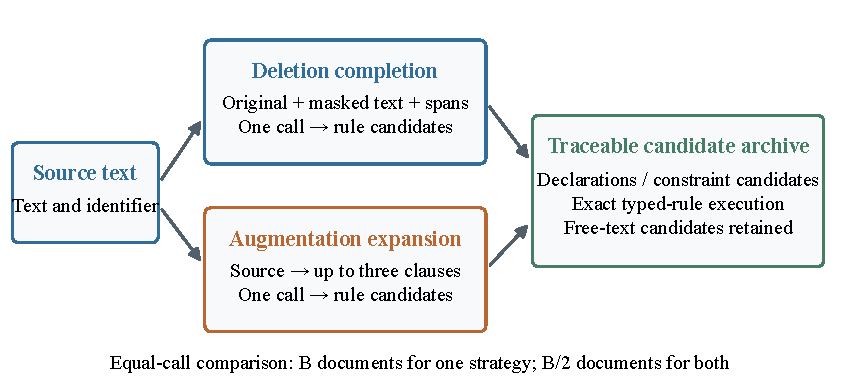
\includegraphics[width=0.96\textwidth]{figure/method/dual_strategy.pdf}
\caption{Dual-strategy generation and the offline execution audit. Both strategies return the same candidate categories. Exact typed constraints can be executed directly; free-text candidates remain in the archive for further validation.}
\label{fig:dual_strategy}
\end{figure*}

\subsubsection{Rule Materialization and Validation}
\label{subsubsec:rule_materialization}
A candidate is not automatically an executable or correct rule. We preserve the source document, strategy, response line, candidate category, and ordinal position. The direct execution audit supports explicit triples of subject type, relation, and object type. A forbidden pattern $r=(\tau_s,p,\tau_o)$ flags a record $x$ when
\begin{equation}
V_r(x)=\mathbf1[(\operatorname{type}(s_x),p_x,\operatorname{type}(o_x))=r].
\end{equation}
An allowed pattern records permission for that exact combination. Absence from the allowed set does not imply a violation. When both allowed and forbidden patterns match, the audit records a conflict and abstains. Only outer whitespace is trimmed; no aliases or semantic rewrites are inferred.

Each malformed candidate, unsupported family, unmapped vocabulary item, and unmatched executable pattern remains in the audit. The executable subset is checked on RuleTest-94 using its stored expected outcomes. These labels describe the designed suite and provide an execution check, not independent adjudication of generated rule meaning. The procedural and structural family detectors are a separate hand-implemented comparison and are not attributed to individual generated candidates.

\subsubsection{Aggregation and Provenance}
Candidates are deduplicated within category by the stored aggregation code and canonical serialization. Entity and relation declarations are distinguished from constraints. The replay uses category-level canonical deduplication; it makes no additional semantic merges.

The generation script defaults to Qwen3-32B and temperature 0.2. Per-call records do not preserve a complete run configuration, exact rendered prompt, or decoding metadata. We therefore report those values as script defaults, not verified settings for every historical call. The prompt builders and translated templates are documented in Appendix~\ref{app:prompts}; literal templates are included in the supplementary artifact. The independent extraction benchmark uses Qwen3.8-27B-no-thinking and is separate from rule generation.

\subsection{Offline Generated-Rule Bridge}
\label{sec:rule_bridge_method}
The bridge compiles archived allowed and forbidden typed patterns using the
same exact-match semantics as the execution audit. Activation changes the
current violation report and enables a removal action when an unopposed
forbidden pattern matches a record. After removal, the bridge recomputes
matches and action availability. Every match retains its rule identifier and
source lineage. Unsupported candidates are logged; conflicting permissions
and prohibitions cause abstention.

This prototype uses government-domain typed records rather than mapping the
archive's vocabulary to TNEWS. Its fixed acquisition schedule exercises the
interfaces without training another policy. It removes prohibited records
but does not infer replacement facts; reference labels are used only to
count defective and clean removals after execution.
